\documentclass[../main.tex]{subfiles}

\begin{document}
The thesis focuses on implementing a safe learning controller for an inverted pendulum. Initially, a Markov Decision Process model of the pendulum system is obtained by essentially discretizing the state and action space, assigning rewards to the discrete states, and calculating transition probabilities between the states. As in \cite{akametalu2014reachability}, a system with an unknown additive state-dependent disturbance $d(x)$ is assumed. Additionally, conservative initial disturbance bounds, the upper bound $\overline{d}_0$ and the lower bound $\underline{d}_0$, are assumed to be known initially. The bounds will be iteratively updated with a GP model. Based on the initial disturbance estimate and a safe set, the backwards reachable set, which should be avoided in order to never leave the safe set, is calculated with HJI reachability analysis. This calculation gives rise to a safe region within the state space within which the learning controller can operate freely. Additionally, the safe set calculations output a safe controller that should be applied at the borders of this set. Based on that, the chosen reinforcement learning algorithm can learn a policy by choosing actions and receiving subsequently information about the reward and the state transition associated with that action. If the chosen action would cause the system to leave the safe region, the safe controller acts and brings the system back into the safe set. The chosen reinforcement learning algorithm is a modified version of Delayed Q-Learning introduced in Section \ref{sec:RL}.

While the learning controller acts, data samples are recorded and subsequently fed into the GP model. The GP estimates a less conservative bound for the disturbance so that subsequently a larger safe set can be calculated with HJI reachability analysis. This procedure is sketched in Figure \ref{fig:flow_simple}. The estimated safe set is fed into the safe learning controller that learns a policy through interaction with the system. The samples recorded during learning are used to get a better estimate of the disturbance thus resulting in a less restrictive safe control.\par
\begin{figure}
    \centering
    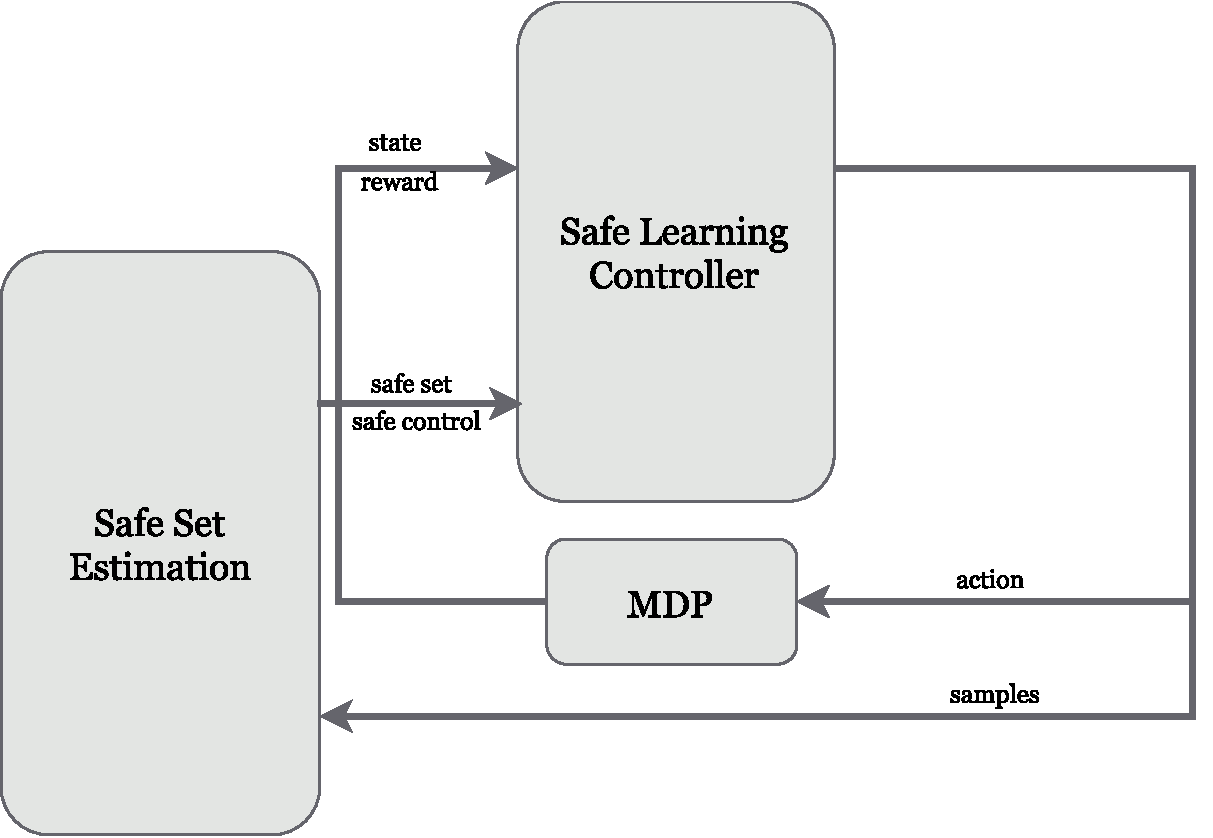
\includegraphics[width=\textwidth]{flow_simple}
    \caption{Rough Control Setup.}
    \label{fig:flow_simple}
\end{figure}
More precisely, the same control scheme is explained in Figure \ref{fig:flow_complete}. In this figure the colours blue and red are used to underline the two control loops that run in parallel: The blue loop is the safety loop, which estimates the disturbance, calculates a safe set (and a safe controller on that basis), and checks every action that the learning controller wants to take. The red loop is the learning control loop where the reinforcement learning controller chooses an action based on its policy, and subsequently receives some feedback from the process. Based on the received reward, the controller updates its policy. For each action chosen by the learning controller, the safe controller performs a check if that action would violate the boundaries of the safe set. If that is the case, the action is not executed but replaced by a safety-preserving action.
\begin{figure}
    \centering
    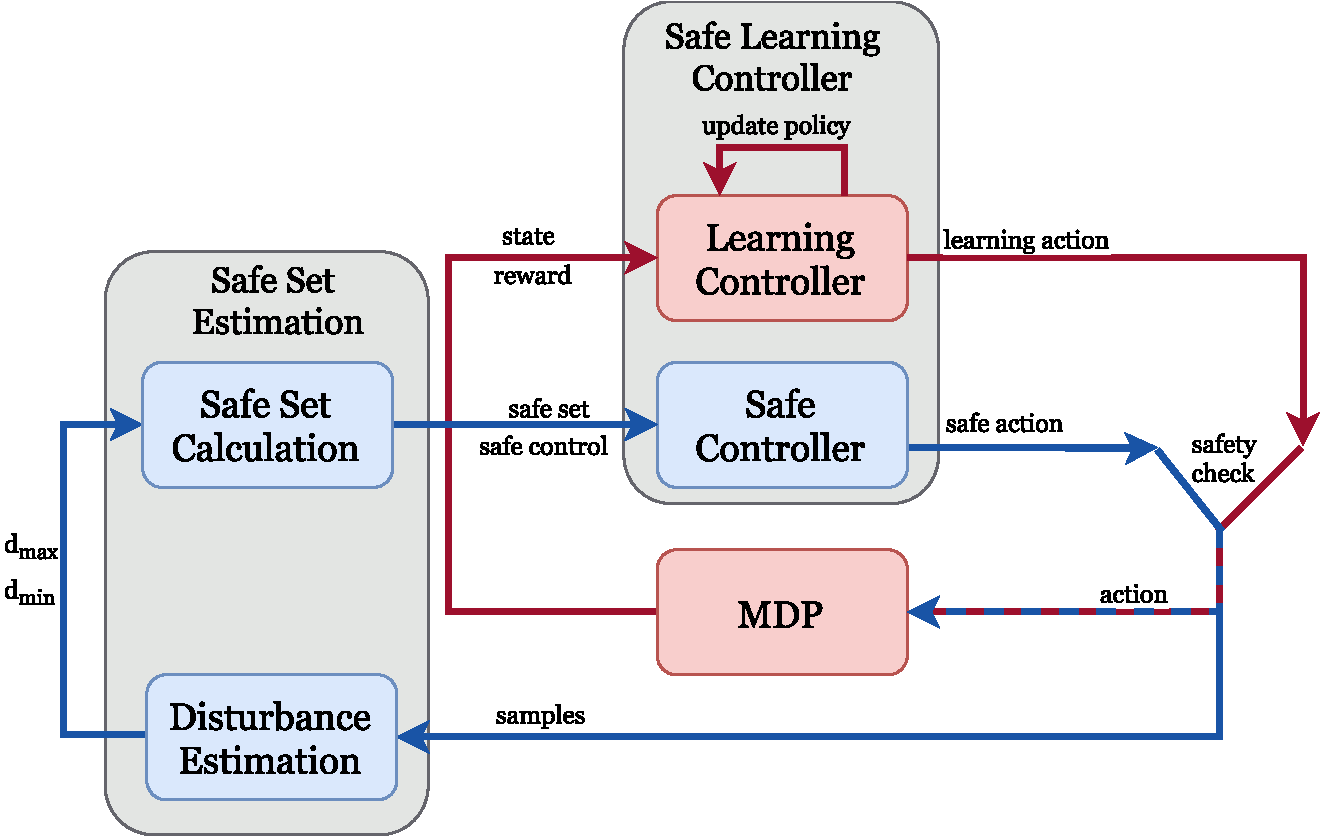
\includegraphics[width=\textwidth]{flow_complete}
    \caption{Detailed Control Setup.}
    \label{fig:flow_complete}
\end{figure}
This very rough sketch will be further explained in Section \ref{sec:Implementation}.

\end{document}